\chapter{Organisation du projet}

\section{Présentation du projet}

En lien avec l'équipe ESTER, nous avons reçu pour objectif de réaliser un site web permettant de créer des questionnaires médicaux auxquels pourraient répondre les salariés de diverses entreprises. Selon le cahier des charges et tout en respectant le secret professionnel, nous devions faire en sorte que les patients (salariés) puissent répondre aux questions que les médecins auraient préparé dans des questionnaires, enregistrés dans une base de données. Une fois créé et enregistré, le corps médical devait pouvoir les attribuer en fonction des cas. Par la suite, des résultats devaient être calculés et affichés aux personnels soignant afin qu'ils puissent se rendre compte des chiffres. 

\section{Choix technologiques}

\subsection{Technologies côté serveur}

\begin{description}

\item[NodeJS] : NodeJS permet de créer des services web en utilisant du JavaScript. 
NodeJS est une technologie moderne avec beaucoup de documentation récente. Elle permet de n'utiliser quasiment que du JavaScript. NodeJS est quelque peu complexe car il utilise un mécanisme de callback et de promesses. Ils sont dûs au fonctionnement asynchrone de NodeJS qui rend le tout très performant.

\item[JEE] : JEE est la version de Java orienté pour la création d'application pour les entreprises et permet de développer des services web.
JEE présente l'avantage d'être simple, car il utilise des mécaniques proche de celle du Java que nous connaissons. 

\end{description}

Nous avons proposé d'utiliser NodeJS côté serveur, mais nos chefs de projet ont privilégié l'utilisation de JEE car c'est une technologie qu'ils connaissaient et qui nous sera utile lors du prochain semestre. Ils estimaient, par ailleurs, qu'il s'agissait d'une solution facile à apprendre, en comparaison de NodeJS. 

\subsection{Technologies côté client}

\begin{description}

\item[JavaScript] : JavaScript est un langage de programmation développé par Netscape en 1995 sous le nom de LiveScript. Il s'agit d'un langage de script léger, orienté objet, principalement connu comme le langage de script des pages web. 
JS nous permet d'effectuer des opérations côté client, modifier l'affichage ou lier des fonctions avec des boutons.\

\item[CSS] : « Cascading Style Sheets » ce qui signifie « feuille de style en cascade ». 
Il s'agit d'un langage informatique utilisé pour mettre en forme les fichiers HTML ou XML. 
CSS permet de modifier l'affichage pour mieux correspondre aux besoins du client, en plus de Bootstrap qui a déjà un CSS de défini. Il permet d'améliorer la qualité visuelle de l'interface utilisateur. \

\item[Bootstrap] : Correspond à une collection d'outils, développée depuis 2010, utiles pour la création de sites web. Cette collection contient des codes HTML et CSS ainsi que des extensions JavaScript. 
Il nous permet d'avoir un aspect unifié et de faciliter le mise en place de page adaptatif entre les différents mobiles et les ordinateurs. Nous avons été amenés à utiliser Bootstrap lors de nos diverses travaux.  \

\item[Highcharts] : Highcharts est une librairie JavaScript qui permet de générer des graphiques interactifs. Le projet nous demandait une certaine mise en forme des résultats. Les paramétrages s'effectuent en JSON et offrent la possibilité d'exporter dans les différents formats CSV, PDF, PNG et autres ainsi qu'être compatible avec les PCs/Tablettes/Smartphones.
Nous l'avons choisi pour sa facilité à exporter les données et car il proposait des exemples pour faciliter son intégration.

\end{description}

\subsection{Base de données}

Pour le projet, nous avons eu besoin d'une base de données modulaire car un des besoins était que les questionnaires pouvaient évoluer : création, modification ou suppression de questions. Un autre des besoins était que l'utilisateur puisse faire des sauvegardes partielles pour reprendre le questionnaire en cas de problème ou si l'utilisateur souhaitait faire une pause. 

En plus des besoins spécifiques pour la sauvegarde des questionnaires et des réponses, il y a des besoins plus génériques comme la gestion des comptes que nous verrons plus en détails dans une autre partie.

\begin{description}

\item[MongoDB] : 
Nous sommes partis sur du MongoDB qui fait partie de la mouvance NoSQL s'écartant du paradigme classique des bases relationnelles. Cela nous permet de nous affranchir d'une des contraintes des bases de données SQL qui est de prévoir un schéma prédéfini. Nous sommes quand même partis d'un schéma de base pour avoir des données en partie structurée.

En offrant une plus grande flexibilité, en permettant de gérer des données non structurées, MongoDB est particulièrement utile pour les questionnaires et les réponses car si un questionnaire est modifié, il était nécessaire que les anciennes réponses restent en partie utilisables.

\begin{figure}[H]
    \begin{center}
    
\includegraphics[height=2.0cm]{img/mongodb}
    \end{center}
    \caption{Logo de MongoDB}
\end{figure}

Ce choix du type de la base de données a été proposé par nos chefs de projet. La raison du choix de MongoDB s'explique par le fait qu'il est le membre le plus sécurisé de la famille NoSQL et facilement maintenable.   

\end{description}

\section{Planification et répartition des tâches}

\subsection{Outils utilisés}

\begin{description}

\item[Github] : 
Git est un outil très utilisé de nos jours dans les entreprises et projets nécessitant un partage de fichiers. Grâce à un espace de stockage à distance et à des fichiers en local, chacun peut travailler sur sa partie et la partager aux autres de manière efficace. Sitôt une partie réalisée, les utilisateurs de Git peuvent envoyer en ligne leurs tâches ce qui permet à leurs collègues de récupérer le code et de l'ajouter au leur par fusion.

\item[Trello] :
Trello est un site internet que nous avons utilisé régulièrement afin de nous attribuer des tâches. Il nous permettait de connaître les parties de chacun et ainsi de mieux nous diriger lorsqu'il était nécessaire de demander des fonctionnalités, les uns les autres.

\item[Slack] :
Nous disposions tout au long du cycle de développement d'un Slack afin d'échanger respectivement nos remarques et interrogations. Toutefois, ne disposant pas d'une version premium, nous ne l'avons pas utilisé pour partager des informations importantes car elles auraient été perdues.

\item[E-mail] :
Comme explicité précédemment, nous n'avons pas pu nous servir de Slack pour échanger de documents importants ou pour garder des conversations importantes. C'est pourquoi nous avons privilégié les adresses e-mails.

\end{description}

\subsection{Diagramme de Gantt}

\begin{figure}[H]
    \begin{center}
    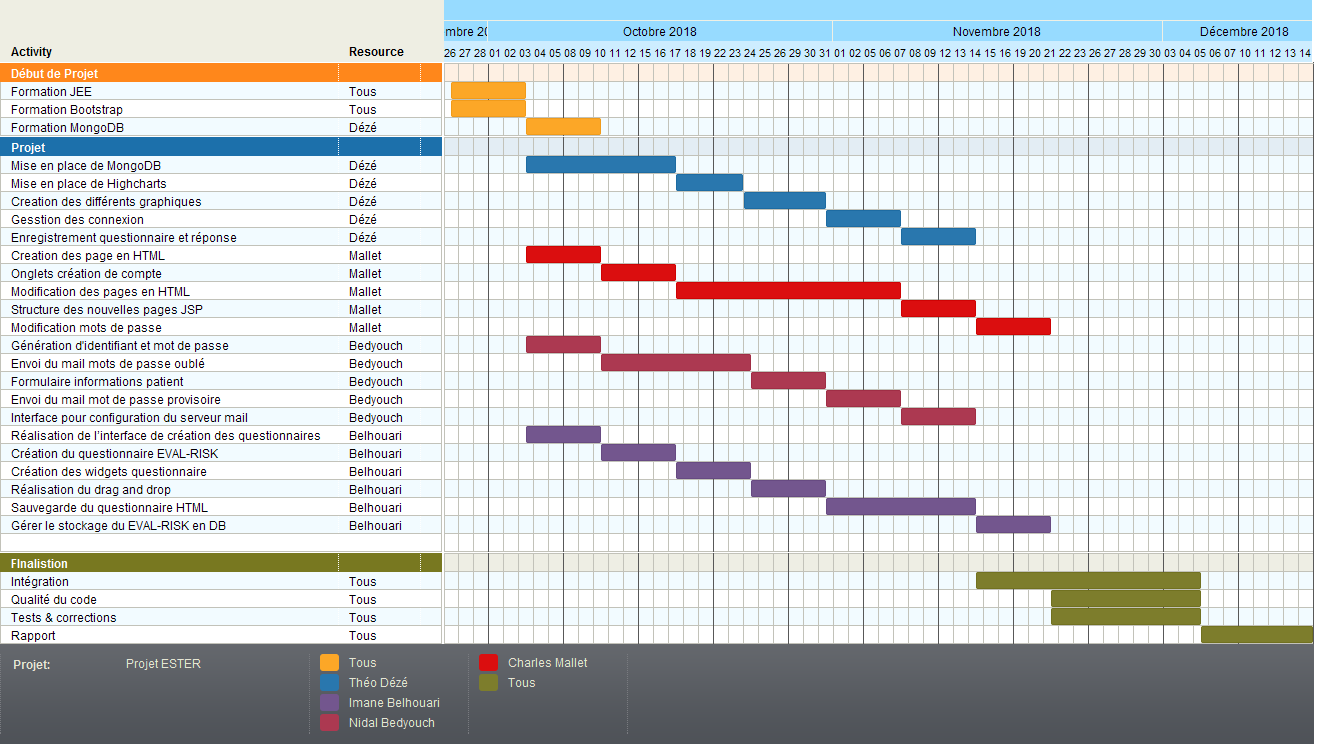
\includegraphics[height=10.0cm]{img/gantt}
    \end{center}
    \caption{Diagramme de Gantt}
\end{figure}

\subsection{Répartitions des rôles}

Nos chefs de projet nous ont demandé dès le début du semestre de leur indiquer nos préférences concernant nos tâches dans le cycle de développement. Imane et Charles se sont occupés principalement du Front-End, Théo et Nidal se sont chargés du Back-End.

Par ailleurs, nos Master 2 souhaitaient que nous nous attribuions un rôle de groupe : 

\begin{description}
\item[Nidal] : Chargée de décisions
\item[Imane] : Chargée d'organisation
\item[Théo] : Référent technique
\item[Charles] : Chargé de communication
\end{description}
